\documentclass{report}

%%%%%%%%%%%%%%%%%%%%%%%%%%%%%%%%%
% PACKAGE IMPORTS
%%%%%%%%%%%%%%%%%%%%%%%%%%%%%%%%%


\usepackage[tmargin=2cm,rmargin=1in,lmargin=1in,margin=0.85in,bmargin=2cm,footskip=.2in]{geometry}
\usepackage{amsmath,amsfonts,amsthm,amssymb,mathtools}
\usepackage[varbb]{newpxmath}
\usepackage{xfrac}
\usepackage[makeroom]{cancel}
\usepackage{mathtools}
\usepackage{bookmark}
\usepackage{enumitem}
\usepackage{hyperref,theoremref}
\hypersetup{
	pdftitle={Assignment},
	colorlinks=true, linkcolor=doc!90,
	bookmarksnumbered=true,
	bookmarksopen=true
}
\usepackage[most,many,breakable]{tcolorbox}
\usepackage{xcolor}
\usepackage{varwidth}
\usepackage{varwidth}
\usepackage{etoolbox}
%\usepackage{authblk}
\usepackage{nameref}
\usepackage{multicol,array}
\usepackage{tikz-cd}
\usepackage[ruled,vlined,linesnumbered]{algorithm2e}
\usepackage{comment} % enables the use of multi-line comments (\ifx \fi) 
\usepackage{import}
\usepackage{xifthen}
\usepackage{pdfpages}
\usepackage{transparent}
\usepackage{youngtab}

\newcommand\mycommfont[1]{\footnotesize\ttfamily\textcolor{blue}{#1}}
\SetCommentSty{mycommfont}
\newcommand{\incfig}[1]{%
    \def\svgwidth{\columnwidth}
    \import{./figures/}{#1.pdf_tex}
}

\usepackage{tikzsymbols}
\renewcommand\qedsymbol{$\Laughey$}


%\usepackage{import}
%\usepackage{xifthen}
%\usepackage{pdfpages}
%\usepackage{transparent}


%%%%%%%%%%%%%%%%%%%%%%%%%%%%%%
% SELF MADE COLORS
%%%%%%%%%%%%%%%%%%%%%%%%%%%%%%



\definecolor{myg}{RGB}{56, 140, 70}
\definecolor{myb}{RGB}{45, 111, 177}
\definecolor{myr}{RGB}{199, 68, 64}
\definecolor{mytheorembg}{HTML}{F2F2F9}
\definecolor{mytheoremfr}{HTML}{00007B}
\definecolor{mylenmabg}{HTML}{FFFAF8}
\definecolor{mylenmafr}{HTML}{983b0f}
\definecolor{mypropbg}{HTML}{f2fbfc}
\definecolor{mypropfr}{HTML}{191971}
\definecolor{myexamplebg}{HTML}{F2FBF8}
\definecolor{myexamplefr}{HTML}{88D6D1}
\definecolor{myexampleti}{HTML}{2A7F7F}
\definecolor{mydefinitbg}{HTML}{E5E5FF}
\definecolor{mydefinitfr}{HTML}{3F3FA3}
\definecolor{notesgreen}{RGB}{0,162,0}
\definecolor{myp}{RGB}{197, 92, 212}
\definecolor{mygr}{HTML}{2C3338}
\definecolor{myred}{RGB}{127,0,0}
\definecolor{myyellow}{RGB}{169,121,69}
\definecolor{myexercisebg}{HTML}{F2FBF8}
\definecolor{myexercisefg}{HTML}{88D6D1}


%%%%%%%%%%%%%%%%%%%%%%%%%%%%
% TCOLORBOX SETUPS
%%%%%%%%%%%%%%%%%%%%%%%%%%%%

\setlength{\parindent}{1cm}
%================================
% THEOREM BOX
%================================

\tcbuselibrary{theorems,skins,hooks}
\newtcbtheorem[number within=section]{Theorem}{Theorem}
{%
	enhanced,
	breakable,
	colback = mytheorembg,
	frame hidden,
	boxrule = 0sp,
	borderline west = {2pt}{0pt}{mytheoremfr},
	sharp corners,
	detach title,
	before upper = \tcbtitle\par\smallskip,
	coltitle = mytheoremfr,
	fonttitle = \bfseries\sffamily,
	description font = \mdseries,
	separator sign none,
	segmentation style={solid, mytheoremfr},
}
{th}

\tcbuselibrary{theorems,skins,hooks}
\newtcbtheorem[number within=chapter]{theorem}{Theorem}
{%
	enhanced,
	breakable,
	colback = mytheorembg,
	frame hidden,
	boxrule = 0sp,
	borderline west = {2pt}{0pt}{mytheoremfr},
	sharp corners,
	detach title,
	before upper = \tcbtitle\par\smallskip,
	coltitle = mytheoremfr,
	fonttitle = \bfseries\sffamily,
	description font = \mdseries,
	separator sign none,
	segmentation style={solid, mytheoremfr},
}
{th}


\tcbuselibrary{theorems,skins,hooks}
\newtcolorbox{Theoremcon}
{%
	enhanced
	,breakable
	,colback = mytheorembg
	,frame hidden
	,boxrule = 0sp
	,borderline west = {2pt}{0pt}{mytheoremfr}
	,sharp corners
	,description font = \mdseries
	,separator sign none
}

%================================
% Corollery
%================================
\tcbuselibrary{theorems,skins,hooks}
\newtcbtheorem[number within=section]{Corollary}{Corollary}
{%
	enhanced
	,breakable
	,colback = myp!10
	,frame hidden
	,boxrule = 0sp
	,borderline west = {2pt}{0pt}{myp!85!black}
	,sharp corners
	,detach title
	,before upper = \tcbtitle\par\smallskip
	,coltitle = myp!85!black
	,fonttitle = \bfseries\sffamily
	,description font = \mdseries
	,separator sign none
	,segmentation style={solid, myp!85!black}
}
{th}
\tcbuselibrary{theorems,skins,hooks}
\newtcbtheorem[number within=chapter]{corollary}{Corollary}
{%
	enhanced
	,breakable
	,colback = myp!10
	,frame hidden
	,boxrule = 0sp
	,borderline west = {2pt}{0pt}{myp!85!black}
	,sharp corners
	,detach title
	,before upper = \tcbtitle\par\smallskip
	,coltitle = myp!85!black
	,fonttitle = \bfseries\sffamily
	,description font = \mdseries
	,separator sign none
	,segmentation style={solid, myp!85!black}
}
{th}


%================================
% LENMA
%================================

\tcbuselibrary{theorems,skins,hooks}
\newtcbtheorem[number within=section]{Lenma}{Lenma}
{%
	enhanced,
	breakable,
	colback = mylenmabg,
	frame hidden,
	boxrule = 0sp,
	borderline west = {2pt}{0pt}{mylenmafr},
	sharp corners,
	detach title,
	before upper = \tcbtitle\par\smallskip,
	coltitle = mylenmafr,
	fonttitle = \bfseries\sffamily,
	description font = \mdseries,
	separator sign none,
	segmentation style={solid, mylenmafr},
}
{th}

\tcbuselibrary{theorems,skins,hooks}
\newtcbtheorem[number within=chapter]{lenma}{Lenma}
{%
	enhanced,
	breakable,
	colback = mylenmabg,
	frame hidden,
	boxrule = 0sp,
	borderline west = {2pt}{0pt}{mylenmafr},
	sharp corners,
	detach title,
	before upper = \tcbtitle\par\smallskip,
	coltitle = mylenmafr,
	fonttitle = \bfseries\sffamily,
	description font = \mdseries,
	separator sign none,
	segmentation style={solid, mylenmafr},
}
{th}


%================================
% PROPOSITION
%================================

\tcbuselibrary{theorems,skins,hooks}
\newtcbtheorem[number within=section]{Prop}{Proposition}
{%
	enhanced,
	breakable,
	colback = mypropbg,
	frame hidden,
	boxrule = 0sp,
	borderline west = {2pt}{0pt}{mypropfr},
	sharp corners,
	detach title,
	before upper = \tcbtitle\par\smallskip,
	coltitle = mypropfr,
	fonttitle = \bfseries\sffamily,
	description font = \mdseries,
	separator sign none,
	segmentation style={solid, mypropfr},
}
{th}

\tcbuselibrary{theorems,skins,hooks}
\newtcbtheorem[number within=chapter]{prop}{Proposition}
{%
	enhanced,
	breakable,
	colback = mypropbg,
	frame hidden,
	boxrule = 0sp,
	borderline west = {2pt}{0pt}{mypropfr},
	sharp corners,
	detach title,
	before upper = \tcbtitle\par\smallskip,
	coltitle = mypropfr,
	fonttitle = \bfseries\sffamily,
	description font = \mdseries,
	separator sign none,
	segmentation style={solid, mypropfr},
}
{th}


%================================
% CLAIM
%================================

\tcbuselibrary{theorems,skins,hooks}
\newtcbtheorem[number within=section]{claim}{Claim}
{%
	enhanced
	,breakable
	,colback = myg!10
	,frame hidden
	,boxrule = 0sp
	,borderline west = {2pt}{0pt}{myg}
	,sharp corners
	,detach title
	,before upper = \tcbtitle\par\smallskip
	,coltitle = myg!85!black
	,fonttitle = \bfseries\sffamily
	,description font = \mdseries
	,separator sign none
	,segmentation style={solid, myg!85!black}
}
{th}



%================================
% Exercise
%================================

\tcbuselibrary{theorems,skins,hooks}
\newtcbtheorem[number within=section]{Exercise}{Exercise}
{%
	enhanced,
	breakable,
	colback = myexercisebg,
	frame hidden,
	boxrule = 0sp,
	borderline west = {2pt}{0pt}{myexercisefg},
	sharp corners,
	detach title,
	before upper = \tcbtitle\par\smallskip,
	coltitle = myexercisefg,
	fonttitle = \bfseries\sffamily,
	description font = \mdseries,
	separator sign none,
	segmentation style={solid, myexercisefg},
}
{th}

\tcbuselibrary{theorems,skins,hooks}
\newtcbtheorem[number within=chapter]{exercise}{Exercise}
{%
	enhanced,
	breakable,
	colback = myexercisebg,
	frame hidden,
	boxrule = 0sp,
	borderline west = {2pt}{0pt}{myexercisefg},
	sharp corners,
	detach title,
	before upper = \tcbtitle\par\smallskip,
	coltitle = myexercisefg,
	fonttitle = \bfseries\sffamily,
	description font = \mdseries,
	separator sign none,
	segmentation style={solid, myexercisefg},
}
{th}

%================================
% EXAMPLE BOX
%================================

\newtcbtheorem[number within=section]{Example}{Example}
{%
	colback = myexamplebg
	,breakable
	,colframe = myexamplefr
	,coltitle = myexampleti
	,boxrule = 1pt
	,sharp corners
	,detach title
	,before upper=\tcbtitle\par\smallskip
	,fonttitle = \bfseries
	,description font = \mdseries
	,separator sign none
	,description delimiters parenthesis
}
{ex}

\newtcbtheorem[number within=chapter]{example}{Example}
{%
	colback = myexamplebg
	,breakable
	,colframe = myexamplefr
	,coltitle = myexampleti
	,boxrule = 1pt
	,sharp corners
	,detach title
	,before upper=\tcbtitle\par\smallskip
	,fonttitle = \bfseries
	,description font = \mdseries
	,separator sign none
	,description delimiters parenthesis
}
{ex}

%================================
% DEFINITION BOX
%================================

\newtcbtheorem[number within=section]{Definition}{Definition}{enhanced,
	before skip=2mm,after skip=2mm, colback=red!5,colframe=red!80!black,boxrule=0.5mm,
	attach boxed title to top left={xshift=1cm,yshift*=1mm-\tcboxedtitleheight}, varwidth boxed title*=-3cm,
	boxed title style={frame code={
					\path[fill=tcbcolback]
					([yshift=-1mm,xshift=-1mm]frame.north west)
					arc[start angle=0,end angle=180,radius=1mm]
					([yshift=-1mm,xshift=1mm]frame.north east)
					arc[start angle=180,end angle=0,radius=1mm];
					\path[left color=tcbcolback!60!black,right color=tcbcolback!60!black,
						middle color=tcbcolback!80!black]
					([xshift=-2mm]frame.north west) -- ([xshift=2mm]frame.north east)
					[rounded corners=1mm]-- ([xshift=1mm,yshift=-1mm]frame.north east)
					-- (frame.south east) -- (frame.south west)
					-- ([xshift=-1mm,yshift=-1mm]frame.north west)
					[sharp corners]-- cycle;
				},interior engine=empty,
		},
	fonttitle=\bfseries,
	title={#2},#1}{def}
\newtcbtheorem[number within=chapter]{definition}{Definition}{enhanced,
	before skip=2mm,after skip=2mm, colback=red!5,colframe=red!80!black,boxrule=0.5mm,
	attach boxed title to top left={xshift=1cm,yshift*=1mm-\tcboxedtitleheight}, varwidth boxed title*=-3cm,
	boxed title style={frame code={
					\path[fill=tcbcolback]
					([yshift=-1mm,xshift=-1mm]frame.north west)
					arc[start angle=0,end angle=180,radius=1mm]
					([yshift=-1mm,xshift=1mm]frame.north east)
					arc[start angle=180,end angle=0,radius=1mm];
					\path[left color=tcbcolback!60!black,right color=tcbcolback!60!black,
						middle color=tcbcolback!80!black]
					([xshift=-2mm]frame.north west) -- ([xshift=2mm]frame.north east)
					[rounded corners=1mm]-- ([xshift=1mm,yshift=-1mm]frame.north east)
					-- (frame.south east) -- (frame.south west)
					-- ([xshift=-1mm,yshift=-1mm]frame.north west)
					[sharp corners]-- cycle;
				},interior engine=empty,
		},
	fonttitle=\bfseries,
	title={#2},#1}{def}



%================================
% Solution BOX
%================================

\makeatletter
\newtcbtheorem{question}{Question}{
	enhanced,
	% breakable,
	colback=white,
	% colframe=myb!80!black,
	% attach boxed title to top left={yshift*=-\tcboxedtitleheight},
	fonttitle=\bfseries,
	title={#2},
	% boxed title size=title,
	% boxed title style={%
	% 		sharp corners,
	% 		rounded corners=northwest,
	% 		colback=tcbcolframe,
	% 		boxrule=0pt,
	% 	},
	% underlay boxed title={%
	% 		\path[fill=tcbcolframe] (title.south west)--(title.south east)
	% 		to[out=0, in=180] ([xshift=5mm]title.east)--
	% 		(title.center-|frame.east)
	% 		[rounded corners=\kvtcb@arc] |-
	% 		(frame.north) -| cycle;
	% 	},
	#1
}{def}
\makeatother

%================================
% SOLUTION BOX
%================================

\makeatletter
\newtcolorbox{solution}{enhanced,
	breakable,
	colback=white,
	colframe=myg!80!black,
	attach boxed title to top left={yshift*=-\tcboxedtitleheight},
	title=Solution,
	boxed title size=title,
	boxed title style={%
			sharp corners,
			rounded corners=northwest,
			colback=tcbcolframe,
			boxrule=0pt,
		},
	underlay boxed title={%
			\path[fill=tcbcolframe] (title.south west)--(title.south east)
			to[out=0, in=180] ([xshift=5mm]title.east)--
			(title.center-|frame.east)
			[rounded corners=\kvtcb@arc] |-
			(frame.north) -| cycle;
		},
}
\makeatother

%================================
% Question BOX
%================================

\makeatletter
\newtcbtheorem{qstion}{Question}{
	% enhanced,
	% breakable,
	% colback=white,
	% colframe=mygr,
	% attach boxed title to top left={yshift*=-\tcboxedtitleheight},
	fonttitle=\bfseries,
	title={#2},
	% boxed title size=title,
	% boxed title style={%
	% 		sharp corners,
	% 		rounded corners=northwest,
	% 		colback=tcbcolframe,
	% 		boxrule=0pt,
	% 	},
	% underlay boxed title={%
	% 		\path[fill=tcbcolframe] (title.south west)--(title.south east)
	% 		to[out=0, in=180] ([xshift=5mm]title.east)--
	% 		(title.center-|frame.east)
	% 		[rounded corners=\kvtcb@arc] |-
	% 		(frame.north) -| cycle;
	% 	},
	#1
}{def}
\makeatother

\newtcbtheorem[number within=chapter]{wconc}{Wrong Concept}{
	breakable,
	enhanced,
	colback=white,
	colframe=myr,
	arc=0pt,
	outer arc=0pt,
	fonttitle=\bfseries\sffamily\large,
	colbacktitle=myr,
	attach boxed title to top left={},
	boxed title style={
			enhanced,
			skin=enhancedfirst jigsaw,
			arc=3pt,
			bottom=0pt,
			interior style={fill=myr}
		},
	#1
}{def}



%================================
% NOTE BOX
%================================

\usetikzlibrary{arrows,calc,shadows.blur}
\tcbuselibrary{skins}
\newtcolorbox{note}[1][]{%
	enhanced jigsaw,
	colback=gray!20!white,%
	colframe=gray!80!black,
	size=small,
	boxrule=1pt,
	title=\textbf{Note:-},
	halign title=flush center,
	coltitle=black,
	breakable,
	drop shadow=black!50!white,
	attach boxed title to top left={xshift=1cm,yshift=-\tcboxedtitleheight/2,yshifttext=-\tcboxedtitleheight/2},
	minipage boxed title=1.5cm,
	boxed title style={%
			colback=white,
			size=fbox,
			boxrule=1pt,
			boxsep=2pt,
			underlay={%
					\coordinate (dotA) at ($(interior.west) + (-0.5pt,0)$);
					\coordinate (dotB) at ($(interior.east) + (0.5pt,0)$);
					\begin{scope}
						\clip (interior.north west) rectangle ([xshift=3ex]interior.east);
						\filldraw [white, blur shadow={shadow opacity=60, shadow yshift=-.75ex}, rounded corners=2pt] (interior.north west) rectangle (interior.south east);
					\end{scope}
					\begin{scope}[gray!80!black]
						\fill (dotA) circle (2pt);
						\fill (dotB) circle (2pt);
					\end{scope}
				},
		},
	#1,
}

%%%%%%%%%%%%%%%%%%%%%%%%%%%%%%
% SELF MADE COMMANDS
%%%%%%%%%%%%%%%%%%%%%%%%%%%%%%


\newcommand{\thm}[2]{\begin{Theorem}{#1}{}#2\end{Theorem}}
\newcommand{\cor}[2]{\begin{Corollary}{#1}{}#2\end{Corollary}}
\newcommand{\mlenma}[2]{\begin{Lenma}{#1}{}#2\end{Lenma}}
\newcommand{\mprop}[2]{\begin{Prop}{#1}{}#2\end{Prop}}
\newcommand{\clm}[3]{\begin{claim}{#1}{#2}#3\end{claim}}
\newcommand{\wc}[2]{\begin{wconc}{#1}{}\setlength{\parindent}{1cm}#2\end{wconc}}
\newcommand{\thmcon}[1]{\begin{Theoremcon}{#1}\end{Theoremcon}}
\newcommand{\ex}[2]{\begin{Example}{#1}{}#2\end{Example}}
\newcommand{\dfn}[2]{\begin{Definition}[colbacktitle=red!75!black]{#1}{}#2\end{Definition}}
\newcommand{\dfnc}[2]{\begin{definition}[colbacktitle=red!75!black]{#1}{}#2\end{definition}}
\newcommand{\qs}[2]{\begin{question}{#1}{}#2\end{question}}
\newcommand{\pf}[2]{\begin{myproof}[#1]#2\end{myproof}}
\newcommand{\nt}[1]{\begin{note}#1\end{note}}

\newcommand*\circled[1]{\tikz[baseline=(char.base)]{
		\node[shape=circle,draw,inner sep=1pt] (char) {#1};}}
\newcommand\getcurrentref[1]{%
	\ifnumequal{\value{#1}}{0}
	{??}
	{\the\value{#1}}%
}
\newcommand{\getCurrentSectionNumber}{\getcurrentref{section}}
\newenvironment{myproof}[1][\proofname]{%
	\proof[\bfseries #1: ]%
}{\endproof}

\newcommand{\mclm}[2]{\begin{myclaim}[#1]#2\end{myclaim}}
\newenvironment{myclaim}[1][\claimname]{\proof[\bfseries #1: ]}{}

\newcounter{mylabelcounter}

\makeatletter
\newcommand{\setword}[2]{%
	\phantomsection
	#1\def\@currentlabel{\unexpanded{#1}}\label{#2}%
}
\makeatother




\tikzset{
	symbol/.style={
			draw=none,
			every to/.append style={
					edge node={node [sloped, allow upside down, auto=false]{$#1$}}}
		}
}


% deliminators
\DeclarePairedDelimiter{\abs}{\lvert}{\rvert}
\DeclarePairedDelimiter{\norm}{\lVert}{\rVert}

\DeclarePairedDelimiter{\ceil}{\lceil}{\rceil}
\DeclarePairedDelimiter{\floor}{\lfloor}{\rfloor}
\DeclarePairedDelimiter{\round}{\lfloor}{\rceil}

\newsavebox\diffdbox
\newcommand{\slantedromand}{{\mathpalette\makesl{d}}}
\newcommand{\makesl}[2]{%
\begingroup
\sbox{\diffdbox}{$\mathsurround=0pt#1\mathrm{#2}$}%
\pdfsave
\pdfsetmatrix{1 0 0.2 1}%
\rlap{\usebox{\diffdbox}}%
\pdfrestore
\hskip\wd\diffdbox
\endgroup
}
\newcommand{\dd}[1][]{\ensuremath{\mathop{}\!\ifstrempty{#1}{%
\slantedromand\@ifnextchar^{\hspace{0.2ex}}{\hspace{0.1ex}}}%
{\slantedromand\hspace{0.2ex}^{#1}}}}
\ProvideDocumentCommand\dv{o m g}{%
  \ensuremath{%
    \IfValueTF{#3}{%
      \IfNoValueTF{#1}{%
        \frac{\dd #2}{\dd #3}%
      }{%
        \frac{\dd^{#1} #2}{\dd #3^{#1}}%
      }%
    }{%
      \IfNoValueTF{#1}{%
        \frac{\dd}{\dd #2}%
      }{%
        \frac{\dd^{#1}}{\dd #2^{#1}}%
      }%
    }%
  }%
}
\providecommand*{\pdv}[3][]{\frac{\partial^{#1}#2}{\partial#3^{#1}}}
%  - others
\DeclareMathOperator{\Lap}{\mathcal{L}}
\DeclareMathOperator{\Var}{Var} % varience
\DeclareMathOperator{\Cov}{Cov} % covarience
\DeclareMathOperator{\E}{E} % expected

% Since the amsthm package isn't loaded

% I prefer the slanted \leq
\let\oldleq\leq % save them in case they're every wanted
\let\oldgeq\geq
\renewcommand{\leq}{\leqslant}
\renewcommand{\geq}{\geqslant}

% % redefine matrix env to allow for alignment, use r as default
% \renewcommand*\env@matrix[1][r]{\hskip -\arraycolsep
%     \let\@ifnextchar\new@ifnextchar
%     \array{*\c@MaxMatrixCols #1}}


%\usepackage{framed}
%\usepackage{titletoc}
%\usepackage{etoolbox}
%\usepackage{lmodern}


%\patchcmd{\tableofcontents}{\contentsname}{\sffamily\contentsname}{}{}

%\renewenvironment{leftbar}
%{\def\FrameCommand{\hspace{6em}%
%		{\color{myyellow}\vrule width 2pt depth 6pt}\hspace{1em}}%
%	\MakeFramed{\parshape 1 0cm \dimexpr\textwidth-6em\relax\FrameRestore}\vskip2pt%
%}
%{\endMakeFramed}

%\titlecontents{chapter}
%[0em]{\vspace*{2\baselineskip}}
%{\parbox{4.5em}{%
%		\hfill\Huge\sffamily\bfseries\color{myred}\thecontentspage}%
%	\vspace*{-2.3\baselineskip}\leftbar\textsc{\small\chaptername~\thecontentslabel}\\\sffamily}
%{}{\endleftbar}
%\titlecontents{section}
%[8.4em]
%{\sffamily\contentslabel{3em}}{}{}
%{\hspace{0.5em}\nobreak\itshape\color{myred}\contentspage}
%\titlecontents{subsection}
%[8.4em]
%{\sffamily\contentslabel{3em}}{}{}  
%{\hspace{0.5em}\nobreak\itshape\color{myred}\contentspage}



%%%%%%%%%%%%%%%%%%%%%%%%%%%%%%%%%%%%%%%%%%%
% TABLE OF CONTENTS
%%%%%%%%%%%%%%%%%%%%%%%%%%%%%%%%%%%%%%%%%%%

\usepackage{tikz}
% \definecolor{doc}{RGB}{0,60,110}
\definecolor{doc}{RGB}{0,0,0}
\usepackage{titletoc}
\contentsmargin{2cm}
\titlecontents{chapter}[4.5pc]
{\addvspace{30pt}%
\pgftext[left,x=-1cm,y=0cm]{\color{black}\Large\sc\bfseries Chapter\ \thecontentslabel}%
	% \begin{tikzpicture}[remember picture, overlay]%
	% 	% \draw[fill=white,draw=white] (0,-.1) rectangle (2,.5);%
	% \end{tikzpicture}\color{black}\large\sc\bfseries
	}%
{}
{}
{\;\hfill\large\sc\bfseries Page \thecontentspage
% 	\begin{tikzpicture}[remember picture, overlay]
% 		\draw[fill=doc!60,draw=doc!60] (2pt,0) rectangle (4,0.1pt);
% 	\end{tikzpicture}}%
}
\titlecontents{section}[0pc]
{\addvspace{2pt}}
{\contentslabel[\thecontentslabel]{2pc}}
{}
{\hfill\small \thecontentspage}
[]
% \titlecontents*{subsection}[3.7pc]
% {\addvspace{-1pt}\small}
% {}
% {}
% {\ \small\thecontentspage}
% [ \textbullet\ ][]

\makeatletter
\renewcommand{\tableofcontents}{%
	\chapter*{%
	  \vspace*{-20\p@}%
	  \begin{tikzpicture}[remember picture, overlay]%
		  \pgftext[left,x=0cm,y=0.2cm]{\color{black}\Huge\sc\bfseries \contentsname};%
		%   \draw[fill=black,draw=black] (13,-.75) rectangle (20,1);%
		%   \clip (13,-.75) rectangle (20,1);
		%   \pgftext[right,x=15cm,y=0.2cm]{\color{black}\Huge\sc\bfseries \contentsname};%
	  \end{tikzpicture}}%
	\@starttoc{toc}}
\makeatother

%From M275 "Topology" at SJSU
\newcommand{\id}{\mathrm{id}}
\newcommand{\taking}[1]{\xrightarrow{#1}}
\newcommand{\inv}{^{-1}}

%From M170 "Introduction to Graph Theory" at SJSU
\DeclareMathOperator{\diam}{diam}
\DeclareMathOperator{\ord}{ord}
\newcommand{\defeq}{\overset{\mathrm{def}}{=}}

%From the USAMO .tex files
\newcommand{\ts}{\textsuperscript}
\newcommand{\dg}{^\circ}
\newcommand{\ii}{\item}

% % From Math 55 and Math 145 at Harvard
\newenvironment{subproof}[1][Proof]{%
\begin{proof}[#1] \renewcommand{\qedsymbol}{$\blacksquare$}}%
{\end{proof}}

\newcommand{\liff}{\leftrightarrow}
\newcommand{\lthen}{\rightarrow}
\newcommand{\opname}{\operatorname}
\newcommand{\surjto}{\twoheadrightarrow}
\newcommand{\injto}{\hookrightarrow}
\newcommand{\On}{\mathrm{On}} % ordinals
\DeclareMathOperator{\img}{im} % Image
\DeclareMathOperator{\Img}{Im} % Image
\DeclareMathOperator{\coker}{coker} % Cokernel
\DeclareMathOperator{\Coker}{Coker} % Cokernel
\DeclareMathOperator{\Ker}{Ker} % Kernel
\DeclareMathOperator{\rank}{rank}
\DeclareMathOperator{\Spec}{Spec} % spectrum
\DeclareMathOperator{\Tr}{Tr} % trace
\DeclareMathOperator{\pr}{pr} % projection
\DeclareMathOperator{\ext}{ext} % extension
\DeclareMathOperator{\pred}{pred} % predecessor
\DeclareMathOperator{\dom}{dom} % domain
\DeclareMathOperator{\ran}{ran} % range
\DeclareMathOperator{\Hom}{Hom} % homomorphism
\DeclareMathOperator{\Mor}{Mor} % morphisms
\DeclareMathOperator{\End}{End} % endomorphism

\newcommand{\eps}{\epsilon}
\newcommand{\veps}{\varepsilon}
\newcommand{\ol}{\overline}
\newcommand{\ul}{\underline}
\newcommand{\wt}{\widetilde}
\newcommand{\wh}{\widehat}
\newcommand{\vocab}[1]{\textbf{\color{blue} #1}}
\providecommand{\half}{\frac{1}{2}}
\newcommand{\dang}{\measuredangle} %% Directed angle
\newcommand{\ray}[1]{\overrightarrow{#1}}
\newcommand{\seg}[1]{\overline{#1}}
\newcommand{\arc}[1]{\wideparen{#1}}
\DeclareMathOperator{\cis}{cis}
\DeclareMathOperator*{\lcm}{lcm}
\DeclareMathOperator*{\argmin}{arg min}
\DeclareMathOperator*{\argmax}{arg max}
\newcommand{\cycsum}{\sum_{\mathrm{cyc}}}
\newcommand{\symsum}{\sum_{\mathrm{sym}}}
\newcommand{\cycprod}{\prod_{\mathrm{cyc}}}
\newcommand{\symprod}{\prod_{\mathrm{sym}}}
\newcommand{\Qed}{\begin{flushright}\qed\end{flushright}}
\newcommand{\parinn}{\setlength{\parindent}{1cm}}
\newcommand{\parinf}{\setlength{\parindent}{0cm}}
% \newcommand{\norm}{\|\cdot\|}
\newcommand{\inorm}{\norm_{\infty}}
\newcommand{\opensets}{\{V_{\alpha}\}_{\alpha\in I}}
\newcommand{\oset}{V_{\alpha}}
\newcommand{\opset}[1]{V_{\alpha_{#1}}}
\newcommand{\lub}{\text{lub}}
\newcommand{\del}[2]{\frac{\partial #1}{\partial #2}}
\newcommand{\Del}[3]{\frac{\partial^{#1} #2}{\partial^{#1} #3}}
\newcommand{\deld}[2]{\dfrac{\partial #1}{\partial #2}}
\newcommand{\Deld}[3]{\dfrac{\partial^{#1} #2}{\partial^{#1} #3}}
\newcommand{\lm}{\lambda}
\newcommand{\uin}{\mathbin{\rotatebox[origin=c]{90}{$\in$}}}
\newcommand{\usubset}{\mathbin{\rotatebox[origin=c]{90}{$\subset$}}}
\newcommand{\lt}{\left}
\newcommand{\rt}{\right}
\newcommand{\bs}[1]{\boldsymbol{#1}}
\newcommand{\exs}{\exists}
\newcommand{\st}{\strut}
\newcommand{\dps}[1]{\displaystyle{#1}}

\newcommand{\sol}{\setlength{\parindent}{0cm}\textbf{\textit{Solution:}}\setlength{\parindent}{1cm} }
\newcommand{\solve}[1]{\setlength{\parindent}{0cm}\textbf{\textit{Solution: }}\setlength{\parindent}{1cm}#1 \Qed}
% Things Lie
\newcommand{\kb}{\mathfrak b}
\newcommand{\kg}{\mathfrak g}
\newcommand{\kh}{\mathfrak h}
\newcommand{\kn}{\mathfrak n}
\newcommand{\ku}{\mathfrak u}
\newcommand{\kz}{\mathfrak z}
\DeclareMathOperator{\Ext}{Ext} % Ext functor
\DeclareMathOperator{\Tor}{Tor} % Tor functor
\newcommand{\gl}{\opname{\mathfrak{gl}}} % frak gl group
\renewcommand{\sl}{\opname{\mathfrak{sl}}} % frak sl group chktex 6

% More script letters etc.
\newcommand{\SA}{\mathcal A}
\newcommand{\SB}{\mathcal B}
\newcommand{\SC}{\mathcal C}
\newcommand{\SF}{\mathcal F}
\newcommand{\SG}{\mathcal G}
\newcommand{\SH}{\mathcal H}
\newcommand{\OO}{\mathcal O}

\newcommand{\SCA}{\mathscr A}
\newcommand{\SCB}{\mathscr B}
\newcommand{\SCC}{\mathscr C}
\newcommand{\SCD}{\mathscr D}
\newcommand{\SCE}{\mathscr E}
\newcommand{\SCF}{\mathscr F}
\newcommand{\SCG}{\mathscr G}
\newcommand{\SCH}{\mathscr H}

% Mathfrak primes
\newcommand{\km}{\mathfrak m}
\newcommand{\kp}{\mathfrak p}
\newcommand{\kq}{\mathfrak q}

% number sets
\newcommand{\RR}[1][]{\ensuremath{\ifstrempty{#1}{\mathbb{R}}{\mathbb{R}^{#1}}}}
\newcommand{\NN}[1][]{\ensuremath{\ifstrempty{#1}{\mathbb{N}}{\mathbb{N}^{#1}}}}
\newcommand{\ZZ}[1][]{\ensuremath{\ifstrempty{#1}{\mathbb{Z}}{\mathbb{Z}^{#1}}}}
\newcommand{\QQ}[1][]{\ensuremath{\ifstrempty{#1}{\mathbb{Q}}{\mathbb{Q}^{#1}}}}
\newcommand{\CC}[1][]{\ensuremath{\ifstrempty{#1}{\mathbb{C}}{\mathbb{C}^{#1}}}}
\newcommand{\PP}[1][]{\ensuremath{\ifstrempty{#1}{\mathbb{P}}{\mathbb{P}^{#1}}}}
\newcommand{\HH}[1][]{\ensuremath{\ifstrempty{#1}{\mathbb{H}}{\mathbb{H}^{#1}}}}
\newcommand{\FF}[1][]{\ensuremath{\ifstrempty{#1}{\mathbb{F}}{\mathbb{F}^{#1}}}}
% expected value
\newcommand{\EE}{\ensuremath{\mathbb{E}}}
\newcommand{\charin}{\text{ char }}
\DeclareMathOperator{\sign}{sign}
\DeclareMathOperator{\Aut}{Aut}
\DeclareMathOperator{\Inn}{Inn}
\DeclareMathOperator{\Syl}{Syl}
\DeclareMathOperator{\Gal}{Gal}
\DeclareMathOperator{\GL}{GL} % General linear group
\DeclareMathOperator{\SL}{SL} % Special linear group

%---------------------------------------
% BlackBoard Math Fonts :-
%---------------------------------------

%Captital Letters
\newcommand{\bbA}{\mathbb{A}}	\newcommand{\bbB}{\mathbb{B}}
\newcommand{\bbC}{\mathbb{C}}	\newcommand{\bbD}{\mathbb{D}}
\newcommand{\bbE}{\mathbb{E}}	\newcommand{\bbF}{\mathbb{F}}
\newcommand{\bbG}{\mathbb{G}}	\newcommand{\bbH}{\mathbb{H}}
\newcommand{\bbI}{\mathbb{I}}	\newcommand{\bbJ}{\mathbb{J}}
\newcommand{\bbK}{\mathbb{K}}	\newcommand{\bbL}{\mathbb{L}}
\newcommand{\bbM}{\mathbb{M}}	\newcommand{\bbN}{\mathbb{N}}
\newcommand{\bbO}{\mathbb{O}}	\newcommand{\bbP}{\mathbb{P}}
\newcommand{\bbQ}{\mathbb{Q}}	\newcommand{\bbR}{\mathbb{R}}
\newcommand{\bbS}{\mathbb{S}}	\newcommand{\bbT}{\mathbb{T}}
\newcommand{\bbU}{\mathbb{U}}	\newcommand{\bbV}{\mathbb{V}}
\newcommand{\bbW}{\mathbb{W}}	\newcommand{\bbX}{\mathbb{X}}
\newcommand{\bbY}{\mathbb{Y}}	\newcommand{\bbZ}{\mathbb{Z}}

%---------------------------------------
% MathCal Fonts :-
%---------------------------------------

%Captital Letters
\newcommand{\mcA}{\mathcal{A}}	\newcommand{\mcB}{\mathcal{B}}
\newcommand{\mcC}{\mathcal{C}}	\newcommand{\mcD}{\mathcal{D}}
\newcommand{\mcE}{\mathcal{E}}	\newcommand{\mcF}{\mathcal{F}}
\newcommand{\mcG}{\mathcal{G}}	\newcommand{\mcH}{\mathcal{H}}
\newcommand{\mcI}{\mathcal{I}}	\newcommand{\mcJ}{\mathcal{J}}
\newcommand{\mcK}{\mathcal{K}}	\newcommand{\mcL}{\mathcal{L}}
\newcommand{\mcM}{\mathcal{M}}	\newcommand{\mcN}{\mathcal{N}}
\newcommand{\mcO}{\mathcal{O}}	\newcommand{\mcP}{\mathcal{P}}
\newcommand{\mcQ}{\mathcal{Q}}	\newcommand{\mcR}{\mathcal{R}}
\newcommand{\mcS}{\mathcal{S}}	\newcommand{\mcT}{\mathcal{T}}
\newcommand{\mcU}{\mathcal{U}}	\newcommand{\mcV}{\mathcal{V}}
\newcommand{\mcW}{\mathcal{W}}	\newcommand{\mcX}{\mathcal{X}}
\newcommand{\mcY}{\mathcal{Y}}	\newcommand{\mcZ}{\mathcal{Z}}


%---------------------------------------
% Bold Math Fonts :-
%---------------------------------------

%Captital Letters
\newcommand{\bmA}{\boldsymbol{A}}	\newcommand{\bmB}{\boldsymbol{B}}
\newcommand{\bmC}{\boldsymbol{C}}	\newcommand{\bmD}{\boldsymbol{D}}
\newcommand{\bmE}{\boldsymbol{E}}	\newcommand{\bmF}{\boldsymbol{F}}
\newcommand{\bmG}{\boldsymbol{G}}	\newcommand{\bmH}{\boldsymbol{H}}
\newcommand{\bmI}{\boldsymbol{I}}	\newcommand{\bmJ}{\boldsymbol{J}}
\newcommand{\bmK}{\boldsymbol{K}}	\newcommand{\bmL}{\boldsymbol{L}}
\newcommand{\bmM}{\boldsymbol{M}}	\newcommand{\bmN}{\boldsymbol{N}}
\newcommand{\bmO}{\boldsymbol{O}}	\newcommand{\bmP}{\boldsymbol{P}}
\newcommand{\bmQ}{\boldsymbol{Q}}	\newcommand{\bmR}{\boldsymbol{R}}
\newcommand{\bmS}{\boldsymbol{S}}	\newcommand{\bmT}{\boldsymbol{T}}
\newcommand{\bmU}{\boldsymbol{U}}	\newcommand{\bmV}{\boldsymbol{V}}
\newcommand{\bmW}{\boldsymbol{W}}	\newcommand{\bmX}{\boldsymbol{X}}
\newcommand{\bmY}{\boldsymbol{Y}}	\newcommand{\bmZ}{\boldsymbol{Z}}
%Small Letters
\newcommand{\bma}{\boldsymbol{a}}	\newcommand{\bmb}{\boldsymbol{b}}
\newcommand{\bmc}{\boldsymbol{c}}	\newcommand{\bmd}{\boldsymbol{d}}
\newcommand{\bme}{\boldsymbol{e}}	\newcommand{\bmf}{\boldsymbol{f}}
\newcommand{\bmg}{\boldsymbol{g}}	\newcommand{\bmh}{\boldsymbol{h}}
\newcommand{\bmi}{\boldsymbol{i}}	\newcommand{\bmj}{\boldsymbol{j}}
\newcommand{\bmk}{\boldsymbol{k}}	\newcommand{\bml}{\boldsymbol{l}}
\newcommand{\bmm}{\boldsymbol{m}}	\newcommand{\bmn}{\boldsymbol{n}}
\newcommand{\bmo}{\boldsymbol{o}}	\newcommand{\bmp}{\boldsymbol{p}}
\newcommand{\bmq}{\boldsymbol{q}}	\newcommand{\bmr}{\boldsymbol{r}}
\newcommand{\bms}{\boldsymbol{s}}	\newcommand{\bmt}{\boldsymbol{t}}
\newcommand{\bmu}{\boldsymbol{u}}	\newcommand{\bmv}{\boldsymbol{v}}
\newcommand{\bmw}{\boldsymbol{w}}	\newcommand{\bmx}{\boldsymbol{x}}
\newcommand{\bmy}{\boldsymbol{y}}	\newcommand{\bmz}{\boldsymbol{z}}

%---------------------------------------
% Scr Math Fonts :-
%---------------------------------------

\newcommand{\sA}{{\mathscr{A}}}   \newcommand{\sB}{{\mathscr{B}}}
\newcommand{\sC}{{\mathscr{C}}}   \newcommand{\sD}{{\mathscr{D}}}
\newcommand{\sE}{{\mathscr{E}}}   \newcommand{\sF}{{\mathscr{F}}}
\newcommand{\sG}{{\mathscr{G}}}   \newcommand{\sH}{{\mathscr{H}}}
\newcommand{\sI}{{\mathscr{I}}}   \newcommand{\sJ}{{\mathscr{J}}}
\newcommand{\sK}{{\mathscr{K}}}   \newcommand{\sL}{{\mathscr{L}}}
\newcommand{\sM}{{\mathscr{M}}}   \newcommand{\sN}{{\mathscr{N}}}
\newcommand{\sO}{{\mathscr{O}}}   \newcommand{\sP}{{\mathscr{P}}}
\newcommand{\sQ}{{\mathscr{Q}}}   \newcommand{\sR}{{\mathscr{R}}}
\newcommand{\sS}{{\mathscr{S}}}   \newcommand{\sT}{{\mathscr{T}}}
\newcommand{\sU}{{\mathscr{U}}}   \newcommand{\sV}{{\mathscr{V}}}
\newcommand{\sW}{{\mathscr{W}}}   \newcommand{\sX}{{\mathscr{X}}}
\newcommand{\sY}{{\mathscr{Y}}}   \newcommand{\sZ}{{\mathscr{Z}}}


%---------------------------------------
% Math Fraktur Font
%---------------------------------------

%Captital Letters
\newcommand{\mfA}{\mathfrak{A}}	\newcommand{\mfB}{\mathfrak{B}}
\newcommand{\mfC}{\mathfrak{C}}	\newcommand{\mfD}{\mathfrak{D}}
\newcommand{\mfE}{\mathfrak{E}}	\newcommand{\mfF}{\mathfrak{F}}
\newcommand{\mfG}{\mathfrak{G}}	\newcommand{\mfH}{\mathfrak{H}}
\newcommand{\mfI}{\mathfrak{I}}	\newcommand{\mfJ}{\mathfrak{J}}
\newcommand{\mfK}{\mathfrak{K}}	\newcommand{\mfL}{\mathfrak{L}}
\newcommand{\mfM}{\mathfrak{M}}	\newcommand{\mfN}{\mathfrak{N}}
\newcommand{\mfO}{\mathfrak{O}}	\newcommand{\mfP}{\mathfrak{P}}
\newcommand{\mfQ}{\mathfrak{Q}}	\newcommand{\mfR}{\mathfrak{R}}
\newcommand{\mfS}{\mathfrak{S}}	\newcommand{\mfT}{\mathfrak{T}}
\newcommand{\mfU}{\mathfrak{U}}	\newcommand{\mfV}{\mathfrak{V}}
\newcommand{\mfW}{\mathfrak{W}}	\newcommand{\mfX}{\mathfrak{X}}
\newcommand{\mfY}{\mathfrak{Y}}	\newcommand{\mfZ}{\mathfrak{Z}}
%Small Letters
\newcommand{\mfa}{\mathfrak{a}}	\newcommand{\mfb}{\mathfrak{b}}
\newcommand{\mfc}{\mathfrak{c}}	\newcommand{\mfd}{\mathfrak{d}}
\newcommand{\mfe}{\mathfrak{e}}	\newcommand{\mff}{\mathfrak{f}}
\newcommand{\mfg}{\mathfrak{g}}	\newcommand{\mfh}{\mathfrak{h}}
\newcommand{\mfi}{\mathfrak{i}}	\newcommand{\mfj}{\mathfrak{j}}
\newcommand{\mfk}{\mathfrak{k}}	\newcommand{\mfl}{\mathfrak{l}}
\newcommand{\mfm}{\mathfrak{m}}	\newcommand{\mfn}{\mathfrak{n}}
\newcommand{\mfo}{\mathfrak{o}}	\newcommand{\mfp}{\mathfrak{p}}
\newcommand{\mfq}{\mathfrak{q}}	\newcommand{\mfr}{\mathfrak{r}}
\newcommand{\mfs}{\mathfrak{s}}	\newcommand{\mft}{\mathfrak{t}}
\newcommand{\mfu}{\mathfrak{u}}	\newcommand{\mfv}{\mathfrak{v}}
\newcommand{\mfw}{\mathfrak{w}}	\newcommand{\mfx}{\mathfrak{x}}
\newcommand{\mfy}{\mathfrak{y}}	\newcommand{\mfz}{\mathfrak{z}}

\title{\Huge{MATH 413}\\Introduction to Combinatorics}
\author{\huge{Amit Sawhney}}
\date{Fall 2022}

\begin{document}

\maketitle
\newpage% or \cleardoublepage
% \pdfbookmark[<level>]{<title>}{<dest>}
\pdfbookmark[section]{\contentsname}{toc}
\tableofcontents
\pagebreak

\chapter{What is Combinatorics?}

\chapter{Permutations and Combinations}

\section{Lecture 2: Four Basic Counting Principles}

\section{Lecture 3: Permutations and selections of sets I}

\section{Lecture 4: Permutations and selections of sets II: binomial identities}

\section{Lecture 5: Permutations and Combinations of multisets I}

\section{Lecture 6: Permutations and Combinations of multisets II}

\chapter{The Pigeonhole Principle}

\section{Lecture 7: The pigeonhole principle}

\section{Lecture 8: The strong pigeonhole principle}

\section{Lecture 9: Ramsey Theory}

\setcounter{chapter}{4}

\chapter{The Binomial Coefficients}

\section{Lecture 10: Binomial coefficients and the binomial theorem I}

\section{Lecture 11: Binomial coefficients and the binomial theorem II}

\section{Lecture 12: Binomial coefficients and the binomial theorem III}

\chapter{The Inclusion-Exclusion Principle and Applications}

\section{Lecture 13: The Inclusion-Exclusion principle and applications I}

\section{Lecture 14: The Inclusion-Exclusion principle and applications II: Derangements}

\section{Lecture 15: The Inclusion-Exclusion principle and applications II}

\section{Lecture 16: The Inclusion-Exclusion principle and applications IV: Another Forbidden Position Problem}

\chapter{Recurrence Relations and Generating Functions}
\section{Lecture 17: Some Number Sequences}

\ex{Example 1}{
    Consider a configuration of $n$ lines where every two lines
    have a point in common, but no three do. How many regions in the
    plane are there? Give a recurrence. \\

    $$
        a_n = a_{n-1} + n
    $$

    TODO: Give an explanation of why this is true.
}

\ex{Example 2}{
    Give a simple recurrence for dearragements. \\

    $$
        D_n = (n - 1)(D_{n-1} + D_{n-2})
    $$

    TODO: Give an explanation of why this is true. Need to review dearragements
    from previous lecture.
}

\subsubsection*{}
Consider the Fibonacci sequence $f_n = f_{n-1} + f_{n-2}$, where $f_0 = 0$ and $f_1 = 1$.

\dfn{The adjusted Fibonacci sequence: $\hat{F}_n$}{
    This is the number of 1,2 lists of size $n$. In other words,
    consider the number of ways a valet can park A cars (size $1$) and
    B cars (size $2$) in a parking lot of size $n$.

    \begin{equation*}
        \hat{F}_n = \begin{cases}
            1         & \text{if $n = 0$} \\
            f_{n + 1} & \text{otherwise}
        \end{cases}
    \end{equation*}
}

\qs{}{
    Prove
    $$
        \sum_{n=0}^{n} f_{i} = f_{n+2} - 1
    $$
}
\sol{
    \begin{subproof}
        We will prove this by induction on $n$. \\

        \textbf{Base case}: $n = 0$.
        $$
            \sum_{i=0}^{0} f_{i} = f_{0} = 0
        $$

        Similarly,
        $$
            f_{0+2} - 1 = f_{2} - 1 = 1 - 1 = 0
        $$

        So, the base case is true. \\

        \textbf{Inductive Hypothesis}: Assume that the following statement is true for $n = k$.

        $$
            \sum_{i=0}^{k} f_{i} = f_{k+2} - 1
        $$

        \textbf{Indcutive Step}: We will prove that the following statement is true for $n = k + 1$.

        $$
            \sum_{i=0}^{k+1} f_{i} = f_{k+1} + \sum_{i=0}^{k} f_{i} = f_{k+1} + f_{k+2} - 1 = f_{k+3} - 1
        $$

        Therefore, the statement is true for all $n$ by induction.
    \end{subproof}
}

\qs{}{
    Prove
    $$
        1 + \sum_{i=0}^{n} \hat{F}_i = \hat{F}_{n+2}
    $$
}
\sol{
\begin{subproof}
    We will prove this by induction on $n$. \\

    \textbf{Base case}: $n = 0$.
    $$
        1 + \sum_{i=0}^{0} \hat{F}_i = 1 + \hat{F}_0 = 1 + 1 = 2
    $$
    Similarly,
    $$
        \hat{F}_{0+2} = \hat{F}_{2} = f_{2+1} = f_{3} = 2
    $$
    So, the base case is true. \\

    \textbf{Inductive Hypothesis}: Assume that the following statement is true for $n = k$.
    $$
        1 + \sum_{i=0}^{k} \hat{F}_i = \hat{F}_{k+2}
    $$

    \textbf{Inductive Step}: We will prove that the following statement is true for $n = k + 1$.
    \begin{align*}
        1 + \sum_{i=0}^{k+1} \hat{F}_i & = 1 + \hat{F}_{k+1} + \sum_{i=0}^{k} \hat{F}_i \\
                                       & = \hat{F}_{k+1} + \hat{F}_{k+2}                \\
                                       & = f_{k+2} + f_{k+3}                            \\
                                       & = f_{k+4}                                      \\
                                       & = \hat{F}_{k+3}                                \\
    \end{align*}

    Therefore, the statement is true for all $n$ by induction.
\end{subproof}

\qs{}{
    Prove that $f_n$ is even if and only if $n$ is divisible by $3$.
}
\sol{
    \begin{subproof}
        Given that $f_0 = 0$, $f_1 = 1$, and $f_2 = 1$, we can see that
        at $n = 3$, $f_3 = 2$, which is even. \\

        This is because the only way to get an even number is to have
        the parity of the two numbers added togethed (odd + odd or even + even)
        be the same. So, $f_4$, must be odd, $f_5$ must be odd and
        $f_6$ must be even. \\

        Given the starting sequence of even, odd, odd. The following sequence
        must always be even, odd, odd, which repeats every $3$ numbers.

        Since the first $n = 0$ is the first number in the sequence, every $n$
        that is divisible by $3$ is even.
    \end{subproof}
}
\nt{
    Example problems for later \\

    Guess and prove by induction (you may replace the Fibonnaci
    number by the adjusted Fibonacci number if it helps you) \\

    \begin{itemize}
        \item $f_1 + f_3 + \cdots + f_{2n - 1} = ?$
        \item $f_0 + f_2 + \cdots + f_{2n} = ?$
        \item $f_0 - f_1 + f_2 - \cdots + (-1)^{n}f_n = ?$
        \item $(f_0)^2 + (f_1)^2 + \cdots + (f_n)^2 = ?$
    \end{itemize}
}

\subsubsection*{Obtaining an explicit formula for $f_n$ for linear recurrences}
\ex{}{
    Consider the Fibonacci sequence $f_n = f_{n-1} + f_{n-2}$, where $f_0 = 0$ and $f_1 = 1$.
    This can be rewritten as a linear recurrence as follows:
    $$
        f_n - f_{n-1} - f_{n-2} = 0
    $$

    We must solve the corresponding characterstic equation. Notice how the largest
    degree lines up with the "largest" case of the recurrence. \\

    $$
        x^2 - x - 1 = 0
    $$

    Let $q_1$ and $q_2$ be the roots of the characteristic equation. \\

    It is potentially relevant to note that the following is a solution space
    of the Fibonacci recurrence (but don't satisfy $f_0$ --
    the initial condition): \\

    \begin{equation*}
        \begin{cases}
            q_1^n - q_1^{n - 1} - q_1^{n - 2} = 0 \\
            q_2^n - q_2^{n - 1} - q_2^{n - 2} = 0 \\
        \end{cases}
    \end{equation*}

    The rest of this is based on an ansatz, i.e.
    we need to make an assumption at the answer and validate it later \\

    $$
        f_n = c_1q_1^n + c_2q_2^n,
    $$

    for \textit{some} $c_1, c_2 \in \mathbb{R}$. \\

    Using the initial conditions of $f_0 = 0$ and $f_1 = 1$,
    we can solve for $c_1$ and $c_2$.
}

\section{Lecture 18: Introduction to ordinary generating series}

\nt{
    Up until now, we have solved an instance combinatorial problem at a time.
    However, in some cases, solving a single combinatorial is too difficult.
    So, we solve all of the combinatorial problems at once.
}

\subsubsection*{}
Consider a sequence $$h_0, h_1, h_2, \dots, h_t, \dots$$ of natural numbers where
$h_t$ is the answer to some counting problem that depends on $t$. \\

We can create a generating series of the form:

$$
    g(x) = h_0 + h_1x + h_2x^2 + \cdots + h_tx^t + \cdots
$$

where $h_t = [x^t]g(x)$.

\nt{
    The notation $[x^t]g(x)$ is the coefficient of $x^t$ in the polynomial $g(x)$.
}

\clm{Compositions Generating Series}{}{
    $$
        g(x) = \Big ( \frac{1}{1 - x} \Big )^k
    $$
}

\ex{}{
    Fix $k$. Let \\

    $h_t = $ number of nonnegative integral solutions to
    $$
        e_1 + \cdots + e_k = t, e_i \in \mathbb{Z}_{\ge 0}
    $$

    We already know from stars and bars that

    $$
        h_t = \binom{t + k - 1}{k - 1}
    $$

    So obviously, the generating series can be written as

    $$
        g(x) = \sum_{t=0}^{\infty} \binom{t + k - 1}{k - 1}x^t
    $$

    \nt{
        This doesn't really tell us anything. We just combined some definitions
        and have a genearting series that is hard to utilize in any useful way.
    }

    Take our claim and expand it out with Taylor Series $k$ times:

    \begin{align*}
        g(x) & = \Big ( \frac{1}{1 - x} \Big )^k                                           \\
             & = (1 + x + x^2 + \cdots)(1 + x + x^2 + \cdots)(1 + x + x^2 + \cdots) \cdots \\
    \end{align*}

    We can see that the coefficient of $x^t$ is the number of ways to write $t$ as
    a sum of $k$ nonnegative integers. So,

    $$h_t = \binom{t + k - 1}{k - 1}$$

    This combinatorially proves the negative binomial theorem:

    $$
        g(x) = \Big ( \frac{1}{1 - x} \Big )^k
    $$
}

\subsubsection*{Remark}
If you knew that the negative binomial theorem was true,
you could use it to algebraically solve the composition problem after
choosing the correct generating series $g(x) = \Big ( \frac{1}{1 - x} \Big )^k$.

\qs{}{
    What is

    $$
        (1 + x + x^2 + x^3 + x^4 + x^5)( x + x^2)(1 + x + x^2 + x^3 + x^4)
    $$

    the generating series for?
}
\sol{
    The solutions to the equation

    $$
        e_1 + e_2 + e_3 = t
    $$

    where $0 \le e_1 \le 5, 1 \le e_2 \le 2, 0 \le e_3 \le 4$.
}

\qs{}{
    Suppose you have 1,5 and 25 cents coins available
    (infinite supply). Write down the generating series
    for the number of ways to make change for a dollar.
    How many ways are there?
}
\sol{

    The generating series for the number of ways to make change for an arbitrary amount of money is:

    $$
        g(x) = (1 + x + x^{1+1} + x^{1+1+1} + \cdots)(1 + x^{5} + x^{5+5} + x^{5+5+5} + \cdots)(1 + x^{25} + x^{25+25} + x^{25+25+25} + \cdots)
    $$

    This can be simplified as follows:

    \begin{align*}
        g(x) & = \Big ( \frac{1}{1 - x} \Big ) \Big ( \frac{1}{1 - x^{5}} \Big ) \Big ( \frac{1}{1 - x^{25}} \Big ) \\
             & = \frac{1}{(1 - x)(1 - x^{5})(1 - x^{25})}                                                           \\
    \end{align*}

    The answers is $[x^{100}]g(x)$.
}

\qs{Nonstandard Dice}{
    Compute the generating series for the result of rolling two standard dice. \\
    Now factor it, and interpret.
}
\sol{
    \begin{align*}
        g(x) & = (x + x^2 + x^3 + x^4 + x^5 + x^6)(x + x^2 + x^3 + x^4 + x^5 + x^6) \\
             & = (x + x^2 + x^3 + x^4 + x^5 + x^6)^2                                \\
             & = (1 + x)(1 + x)(x + x^3 + x^5)
    \end{align*}

    TODO: How does this factor like this?

    After factoring, we can see that this is the equivalent of
    flipping a coin twice and rolling two 1-3-5 dice.
}

\qs{}{
    Determine the generating series for partitions.
}
\sol{
    \begin{align*}
        g(x) & = (1 + x^{1} + x^{1+1} + x^{1+1+1} + \cdots)(1 + x^{2} + x^{2+2} + x^{2+2+2} + \cdots)(1 + x^{3} + x^{3+3} + x^{3+3+3} + \cdots) \cdots \\
             & = \Big ( \frac{1}{1 - x} \Big ) \Big ( \frac{1}{1 - x^{2}} \Big ) \Big ( \frac{1}{1 - x^{3}} \Big ) \cdots                              \\
             & = \prod_{i=1}^{\infty} \Big ( \frac{1}{1 - x^{i}} \Big )                                                                                \\
    \end{align*}
}

In words, this generating series is the product of compositions of just $1$'s, $2$'s, $3$'s, etc.

\dfn{Ordinary Generating Series}{
    Let a combinatorial problem be defined as $(S, \omega)$ with $S$ a set
    and $\omega: S \mapsto \mathbb{Z}_{\ge 0}$ The ordinary generating series is

    \begin{align*}
        g(x) = g_{(S, \omega)}(x) = \sum_{s \in S} x^{\omega(s)}
    \end{align*}
}

\thm{Addition Rule of Generating Series}{
    Suppose $S = A \cup B$ (disjoint union), where $(A, \omega_A)$
    and $(B, \omega_B)$ are combinatorial problems.
    Moreover $\omega|_A = \omega_A$ and $\omega|_B = \omega_B$.

    Then the ordinary generating series for $(S, \omega)$ is

    \begin{align*}
        g_{(S, \omega)}(x) & = g_{(A, \omega_A)}(x) + g_{(B, \omega_B)}(x)                     \\
                           & = \sum_{s \in A} x^{\omega_A(s)} + \sum_{s \in B} x^{\omega_B(s)} \\
                           & = \sum_{s \in S} x^{\omega(s)}
    \end{align*}
}

\nt{
    The notation $\omega|_A$ means the restriction of $\omega$ to $A$.
    In this case,

    $$
        \omega|_A = \{ \omega_A(s) \mid s \in A \}
    $$
}

\thm{Product rule of Generating Series}{
    Suppose $S = A \times B$ (cartesian product), where $(A, \omega_A)$
    and $(B, \omega_B)$ are combinatorial problems and

    \begin{align*}
        \omega(a, b) = \omega_A(a) + \omega_B(b)
    \end{align*}

    Then,

    \begin{align*}
        g_{(S, \omega)}(x) & = g_{(A, \omega_A)}(x)g_{(B, \omega_B)}(x)                      \\
                           & = \sum_{a \in A} x^{\omega_A(a)} \sum_{b \in B} x^{\omega_B(b)} \\
                           & = \sum_{a \in A} \sum_{b \in B} x^{\omega(a, b)}
    \end{align*}
}

\subsection*{What does it mean for two generating series to be equal?}

They are equal coefficient by coefficient.

\subsection*{Let $g(x)$ be the ggenerating series for the number of partitions.
    What does it mean that $g(x)$ equals the infinite product:
}

\begin{align*}
    g(x) = \frac{1}{1 - x} \cdot \frac{1}{1 - x^{2}} \cdot \frac{1}{1 - x^{3}} \cdots
\end{align*}

It means that if we expand/solve enough terms of the RHS, the coefficient
of $x^t$ will stabalize (as in no more terms multiplied in will impact
the coefficient) and this coefficient will be the same as the coefficient
of $x^t$ in the LHS -- $g(x)$.

\subsection*{Convergence Issues}

Typically, with generating series, we only care about the coefficients and
not plugging in any specfic value into $x$. Because of this, we do not need
to worry about convergence. However, in some cases $g(x)$ is a polynomial
and in these cases, substitution is fine to perform.

\qs{Substituting into a generating series}{
    Let $S = \{$coins in your pokcet$\}$ and $\omega : S \mapsto \mathbb{Z}_{\ge 0}$
    be the obvious weight function on coins, i.e. $\omega$(nicket)$ = 5$. Is $g(x)$ is
    the corresponding generating series, what is $g(1)$? What is $g'(1)$?
}
\sol{
    $g(1)$ will be the number of coins in your pocket. This is trivially true
    because each term is $x$ to the power of an integer (with no coefficient),
    so $1$ raised to anything will be $1$ and so it is just the number of terms.
    More mathematically,

    \begin{align*}
        g(1) & = \sum_{s \in S} 1^{\omega(s)} \\
             & = \sum_{s \in S} 1             \\
             & = |S|
    \end{align*}

    $g'(1)$ will the amount of money you have. Based on the previous statement,
    we can see that the derivative of $g(x)$ is just the sum of the powers which
    represented the values of the coins in your pocket. More mathematically,
    \begin{align*}
        g'(1) = \sum_{s \in S} \omega(s)
    \end{align*}
}

\chapter{Special Counting Sequences}

\section{Lecture 19: Partition identities}

\dfn{Partition}{
    A \textit{partition} is a decreasing sequence of positive integers whose sum is $n$.
}

\ex{}{
    Consider $n = 5$. The partitions of $5$ are

    \begin{align*}
        & 5 \\
        & 4, 1 \\
        & 3, 2 \\
        & 3, 1, 1 \\
        & 2, 2, 1 \\
        & 2, 1, 1, 1 \\
        & 1, 1, 1, 1, 1
    \end{align*}

    However, this can also be represented in terms of the \textbf{Ferrers diagram}:

    Partitions $5$:

    \begin{align*}
        & \young(~~~~~) \\
        & \young(~~~~,~) \\
        & \young(~~~,~~) \\
        & \young(~~~,~,~) \\
    \end{align*}

    \begin{align*}
        & \young(~~,~~,~) \\
        & \young(~~,~,~,~) \\
        & \young(~,~,~,~,~)
    \end{align*}
}

\ex{Theorem 8.3.1 from the textbook}{
    Use Ferrers diagrams to prove that the number of partitions of $n$ 
    in which the largest part is $r$ equals the number of partitions 
    of $n-r$ in which no part is greater than $r$. \\

    Let $P$ be a partition for $n$. Remove the first part of $P$ which 
    by definition is the largest part which has an arbitrary size $r$. 
    This clearly yields a partition of $n-r$ in which no part is greater
    than $r$. This process is clearly a bijection and so the number of partitions
    of $n$ in which the largest part is $r$ equals the number of partitions
    of $n-r$ in which no part is greater than $r$. \\
}

\nt{
    This process for proving two partitions to be of equal size is important.
}

\subsection*{Generating Series , and partition identities}

Recall generating series for partition: 

\begin{align*}
    g(x) = \prod_{k=1}^{\infty} \Big ( \frac{1}{1 - x^{k}} \Big )
\end{align*}

\qs{}{
    Write down the generating series for:

    \begin{enumerate}
        \item only odd parts
        \item no part repeated more than $m$ times
    \end{enumerate}
}
\sol{Only odd parts:}{
    \begin{align*}
        g(x) &= (1 + x^1 + x^{1+1} + x^{1+1+1} + \cdots) \cdot (1 + x^3 + x^{3+3} + x^{3+3+3} + \cdots) \cdot \cdots \\
             &= \prod_{k=1}^{\infty} \Big ( \frac{1}{1 - x^{2k-1}} \Big )
    \end{align*} 
}

\sol{No part repeated more than $m$ times}{
    \begin{align*}
        g(x) &= (1 + x + x^{1 + 1} + \cdots + x^{m})(1 + x^{2} + x^{2 + 2} + \cdots + x^{2m})(1 + x^{3} + x^{3 + 3} + \cdots + x^{3m}) \cdots \\
             &= (\frac{1}{1 - x} - \frac{x^m}{1 - x}) \cdot (\frac{1}{1 - x^2} - \frac{x^m}{1 - x^2}) \cdot (\frac{1}{1 - x^3} - \frac{x^m}{1 - x^3}) \cdots \\
             &= \prod_{k=1}^{\infty} \Big ( \frac{1}{1 - x^k} - \frac{x^m}{1 - x^k} \Big ) \\
             &= \prod_{k=1}^{\infty} \Big ( \frac{1 - x^m}{1 - x^k} \Big )
    \end{align*}
}

\subsection*{Terminology}

\dfn{Partition size}{
    The \textit{size} of a partition is the sum of its parts.
}

\dfn{Partition length}{
    The \textit{length} of a partition is the number of parts.
}

\qs{}{
    Write down a two variable generating series that counts partitions 
    by both size and length, using say, a $q$ variable and a $z$ variable 
    respectively. Hence the coefficient of $q^nz^l$ is the number of 
    partitions of size $n$ and length $l$.
}
\sol{
    \begin{align*}
        g(q, z) &= \sum_{n=1}^{\infty} \sum_{l=1}^{\infty} P(n,l) \cdot q^{n}z^{l} \\
                &= \prod_{k=0}^{\infty} (1 + zq^{k} + z^2q^{2k} + z^3q^{3k} + \cdots) \\
                &= \prod_{k=0}^{\infty} \Big ( \frac{1}{1 - zq^{k}} \Big )
    \end{align*}
}
\qs{}{
    Consider the identity:

    \begin{align*}
        \prod_{k=1}^{\infty} 1 + q^k = \prod_{k=1}^{\infty} \frac{1}{1 - q^{2k - 1}}
    \end{align*}

    \begin{itemize}
        \item Interpret both sides of the identity. 
        \item Give an algabraic proof.
        \item Can you give a combinatorial proof?
    \end{itemize}
}
\sol{Interpret both sides of the identity}{
    \begin{itemize}
        \item LHS
        
        \begin{align*}
            \prod_{k=1}^{\infty} 1 + q^k = (1 + q^1)(1 + q^2)(1 + q^3) \cdots
        \end{align*}

        This is clearly the number of partitions with distinct parts that 
        are used at most one time.

        \item RHS
        
        This is clearly the generating series for partitions with only odd parts.
    \end{itemize}
}

\sol{Give an algebraic proof}{

\begin{subproof}
    \begin{align*}
        \prod_{k=1}^{\infty} 1 + q^k &= \prod_{k=1}^{\infty} \frac{1-q^k}{1-q^k} (1 + q^k) \\
        &= \prod_{k=1}^{\infty} \frac{1 - q^{2k}}{1 - q^k} \\
        &= \prod_{k=1}^{\infty} \frac{1}{1 - q^k} - \frac{q^{2k}}{1 - q^k} \\
        &= \prod_{k=1}^{\infty} \frac{1}{1 - q^k} - \prod_{k=1}^{\infty} \frac{q^{2k}}{1-q^k} \\
        &= \text{ All partitions - partitions with even parts} \\
        &= \text{ Partitions with odd parts} \\
        &= \prod_{k=1}^{\infty} \frac{1}{1 - q^{2k-1}}
    \end{align*}
\end{subproof}
}

\sol{Give a combinatorial proof}{
    \begin{subproof}
        Fix $n$. Let $S$ be the set of all partitions of $n$ with only 
        distinct parts. Clearly, the LHS represents the generating series that
        counts $S$. \\
    
        Construct a function $f$ from distinct parts to odd parts by dividing 
        each even number by $2$ until every number is odd. This function is 
        clearly well defined as it will only result in odd parts. This must 
        be a bijection because the input to $f$ must have distinct parts so 
        the number of odd parts created is dependent on the even numbers in 
        the input so the output is unique. Lastly, this is clearly reversible
        by taking the largest subset of repeated odd numbers that is a power 
        of $2$ and summing them. \\

        Thus, because we can decompose $S$ into the set of partitions with
        only odd parts through a bijective function and this decomposition 
        is clearly counted by the RHS. Then, it is clear that the LHS and RHS 
        equivalent. 
    \end{subproof}
}

\section{Lecture 20: Partition identities (continued)}

\dfn{Partition Conjugate}{
    The \textit{conjugate} of a partition is the partition associated
    to the transpose of the Ferrers diagram. \\

    \begin{align*}
        \young(~~~~,~~,~)
    \end{align*}

    has a conjugate of

    \begin{align*}
        \young(~~~,~~,~,~)
    \end{align*}
}

\qs{}{
    Use conjugation to prove the following fact: the number of 
    partitions of n with no part bigger than k equals the number 
    of partitions of n with at most k parts. \\

    Determine the generating series for either of the kinds 
    of partitions from the previous problem.
}
\sol{Using conjugation...}{
    \begin{subproof}
        This part is trivially true. If no part is bigger than $k$, then
        the first row in the Ferrers Diagram, which must be the largest row 
        in the diagram, has at most $k$ parts.
    
        By taking the transpose of the first type of parition, we get a 
        partition with at most $k$ parts as the number of parts will be 
        dictated by the first row. 
    
        Thus, the number of partitions of $n$ with no part bigger than $k$
        is the same as the number of partitions of $n$ with at most $k$ parts.
    \end{subproof}
}
\sol{Generating Series}{
    \begin{align*}
        g(x) = &(1 + x + x^{1+1} + \cdots + x^{k}) \\
               &(1 + x^2 + x^{2+2} + \cdots + x^{2k}) \\
               &(1 + x^3 + x^{3+3} + \cdots + x^{3k}) \cdots 
    \end{align*}
    \begin{align*}
        g(x) &= \prod_{i=1}^{\infty} (1 + x^{i} + x^{2i} + \cdots + x^{ki}) \\
             &= \prod_{i=1}^{\infty} \Big ( \frac{1 - x^{ki+1}}{1 - x^{i}} \Big ) 
    \end{align*}
}

\dfn{Durfee Square}{
    A \textit{Durfee square} is the largest square that sits in the NW 
    corner of the Ferrers diagram of a partition. 
}

\qs{}{
    Show that every Ferrers shape uniquely decomposes into 
    $(D_k, A_k, B_k)$ where $D_k$ is a Durfee square of size $k$, 
    $A_k$ is the partition with at most $k$ parts, and $B_k$ is
    a partition with first part of size at most $k$. 
}
\sol{
    Consider an arbitrary partition:

    \begin{align*}
        \young(~~~~,~~,~)
    \end{align*}

    This can obviously be decomoposed into the triple: 

    \begin{align*}
        \Bigg ( \young(~~,~~) , \young(~~) , \young(~) \Bigg )
    \end{align*}

    There are a few cases to consider: 

    \begin{itemize}
        \item First, this is unique. Clearly, this has to be unique 
        because we are not changing any structure from the partition, 
        but rather we are just decomposing it into a triple. So each 
        partition must uniquely map to its own ordered triple. \\
        \item Second, $A_k$ is the partition with at most $k$ parts. $A_k$
        must have at most $k$ because the Durfee square is of size $k$. $A_k$
        cannot be largely than this because it would contradict either 
        the definition of a partition or the definition of a Durfee square. \\
        \item Third, $B_k$ is the partition with first part of size at most $k$.
        This is true because if the first part of $B_k$ is larger than $k$, then
        this would contradict the definition of a Durfee square or a partition. \\
    \end{itemize}

    Thus, we have shown that every partition can be decomposed into a triple.
}

\dfn{Euler-Gauss Identity}{
    \begin{align*}
        \prod_{k=1}^{\infty} \frac{1}{1 - x^k} = 1 + \sum_{j=1}^{\infty} \frac{x^{j^2}}{\Big ( \prod_{t=1}^{j} 1 - x^t \Big )^2}
    \end{align*}
}

\dfn{Self-conjugate Partition}{
    A partition is \textit{self-conjugate} i its transpose shape is the same
    as its original shape (e.g., the partitions (4,1,1,1) and (3,2,1) 
    are self-conjugate, but (3,2) is not).
}

\qs{}{
    Prove that the number of self conjugate partitions of $n$ 
    equals the number of partitions using only distinct odd parts. 
    Then derive an identity.
}
\sol{
    First, we must prove the number of self conjugate partitions of $n$
    equals the number of partitions using only distinct odd parts. This
    can be done by showing a weight preserving bijection between the 
    two sets. \\

    \dfn{Weight-preserving function}{
        Define the following function:

        \begin{align*}
            f : (S, \omega) \mapsto (S', \omega')
        \end{align*}

        such that $\omega : S \mapsto \mathbb{Z}_{\ge 0}$
        and $\omega' : S' \mapsto \mathbb{Z}_{\ge 0}$ are weight functions. 
        Then, $f$ is a weight-preserving function if and only if:

        \begin{align*}
            \omega(s) = \omega'(f(s)) \text{ for all } s \in S
        \end{align*}
    }

    And so, we can make the following claim

    \clm{}{}{
        If $f : (S, \omega) \mapsto (S', \omega')$ is a weight-preserving
        and bijective  then, 

        \begin{align*}
            g_{(S, \omega)}(x) = g_{(S', \omega')}(x) \in \mathbb{Z}[x]
        \end{align*}

        In other words, their generating functions are equal.
    }

    Now to define the actual bijection. Consider each row of the Ferrers
    diagram of an arbitrary distinct odd partition. Each row can be 
    bent into a self-conjugate partition. By selecting the middle element,
    which is gaurunteed to exist because the partition is odd, we can 
    place every square to the left below the middle element and leave
    the other elements alone. Additionally, this is well defined as each
    row is distinct. Thus, we have a weight preserving bijection 
    between the set of distinct odd partitions and the set 
    of self-conjugate partitions. \\

    The generating function for the number of distinct odd partitions 
    is trivial and given by: 

    \begin{align*}
        g(x) = \prod_{i=1}^{\infty} 1 - x^{2i-1}
    \end{align*}

    as we only want to either select an odd number or not. \\

    The generating function for the number of self-conjugate partitions
    is more complicated. Consider an arbitrary self-conjugate partition
    $\lambda$. We can decompose it into a triple $(D_k, A_k, B_k)$ through
    the Durfee square decomposition. We can then apply a second weight-preserving
    bijection and conjugate the second component of the triple which makes 
    $A_k = B_k$. Lastly, we can apply a third weight-preserving bijection
    by compressing the triple into a tuple $(D_k, C_k)$ where $C_k$ is 
    $A_k$ merged left-to-right with $B_k$. \\

    Consequently, 

    \begin{align*}
        C_k \in \bigcup_{j=0}^{\infty} D_j \times \text{Partitions}_{\text{even}_{\le j \text { tall}}} = U
    \end{align*}

    Clearly, 
    
    \begin{align*}
        g_{U}(x) &= \sum_{j=0}^{\infty} x^{j^2} \Big ( \prod_{t=1}^{j} \frac{1}{1 - x^{2t}} \Big ) \\
                 &= \sum_{j=0}^{\infty} \frac{x^{j^2}}{\prod_{t=1}^{j} \frac{1}{1 - x^{2t}}}
    \end{align*}

    So, 

    \begin{align*}
        \prod_{k=1}^{\infty} 1 + x^{2k - 1} = \sum_{j=0}^{\infty} \frac{x^{j^2}}{\prod_{t=1}^{j} \frac{1}{1 - x^{2t}}}
    \end{align*}


\section{Lecture 21: Exponential generating series}

\chapter*{Midterm 3}
}

\end{document}